\section{Combinatorics}

The definitions come from~\cite{polytopes}

\begin{definition}[Equality relation]
  An equality relation $\sim$ on a set $E$ is a subset $R$ of $E \times E$. We write $x \sim y$ iff $(x,y) \in R$ with the following properties:
  \begin{enumerate}
    \item ("Reflexivity") $x \sim x \ \forall x \in E$
    \item ("Symmetry") $x \sim y \Leftrightarrow y\sim x \ \forall x,y \in E$.
    \item ("Transitivity") if $x \sim y$ and $y \sim z$ then $x \sim z$ for all $x,y,z \in E$.
  \end{enumerate}
\end{definition}

\subsection{Posets}

\begin{definition}[Partially ordered set]
  \index{partially ordered set}
  \index{poset}
  A \textit{partially ordered set} or \textit{poset} is a pair $(P,\le)$ with $P$ a set and $\le$ a relation between $P$ and $P$ such that
  \begin{enumerate}
    \item $x \le x$ ($\forall x \in P$)
    \item ("Anti-symmetry") if $x \le y$ and $y \le x$, then $x = y$ ($\forall x,y \in P$)
    \item ("Transitivity") if $x \le y$ and $y \le z$, then $x \le z$ ($\forall x,y,z \in P$)
  \end{enumerate}
\end{definition}

\paragraph{}
This is called a \textit{partial} order because there is no constraint that implies that every pair of elements of $P$ is comparable, i.e. for $x,y \in P$ it is possible that neither $x \le y$ nor $y \le x$.

\paragraph{}
We denote $x < y$ when $x \le y$ and $x \neq y$.

\paragraph{}
\index{Hasse diagram}
Given a poset, we can draw its Hasse diagram. It's a graph where the vertices are the elements of $P$ and two elements $x$ and $y$ are connected with $x$ under $y$ if $x \le y$. Therefore, no horizontal edge can exist.

\paragraph{}
We try to minimize the number of edges so we will not connect $x$ and $z$ (with $x \le z$) if there exists $y$ such that $x < y < z$. This is required otherwise the diagram becomes overloaded even more quickly. The reader can deduce the removed edge by transitivity.

\begin{figure}[H]
  \begin{center}
    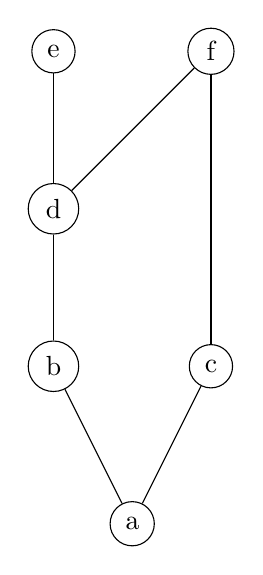
\begin{tikzpicture}

      \begin{scope}[every node/.style={circle,draw}]
        \node (f)  at (2,6)  {f};
        \node (e)  at (0,6)  {e};
        \node (d)  at (0,4)  {d};
        \node (c)  at (2,2)  {c};
        \node (b)  at (0,2)  {b};
        \node (a)  at (1,0)  {a};
      \end{scope}

      \begin{scope}[every node/.style={fill=white,circle}]

        \begin{scope}[every edge/.style={draw}]
          \path (a)  edge (b);
          \path (a)  edge (c);
          \path (b)  edge (d);
          \path (d)  edge (e);
          \path (d)  edge (f);
          \path (c)  edge (f);
        \end{scope}
      \end{scope}

    \end{tikzpicture}
    \caption{Simple Hasse diagram}
  \end{center}
\end{figure}

\paragraph{}
In the figure, there is a link between $a$ and $b$ so $a \le b$, and $b \le d$. So $a \le d$ by transitivity, even if there is no line between those points.

\begin{definition}[Totally ordered set]
  \index{totally ordered set}
  A \textit{totally ordered set} is a poset such that $\forall x,y \in P$, we have $x \le y$ or $y \le x$.
\end{definition}

\begin{definition}[Chain]
  \index{chain}
  A \textit{chain} is a totally ordered subset of a poset.
\end{definition}

\begin{definition}[Interval]
  \index{interval}
\end{definition}

\begin{definition}[Maximal chain]
  A chain is called \textit{maximal} if it is not contained in any bigger chain.
\end{definition}

\subsection{Lattice}

\begin{definition}[Upper bound, Lower bound]
  \index{upper bound}
  \index{lower bound}
  An upper (resp. lower) bound of two elements $x$ and $y$ is an element $m$ such that $x \le m$ and $y \le m$ (resp. $m \le x$ and $m \le y$).
\end{definition}

\begin{definition}[Supremum, Infinimum]
  \index{supremum}
  \index{infinimum}
  The supremum (resp. infinimum) of two elements $x$ and $y$ is the lower (resp. upper) bound of all upper (resp. lower) bounds of $x$ and $y$. If it exists, it's unique. We denote the supremum of $x$ and $y$ $x \wedge y$, and the infinimum $ x \vee y$.
\end{definition}

\begin{definition}[Lattice]
  \index{lattice}
  A lattice is a poset such that every pair of elements has a supremum and an infinimum.
\end{definition}

\paragraph{}
It's not always clear whether a poset is a lattice or not, see for example the following diagram.

\begin{figure}[H]
  \begin{center}
    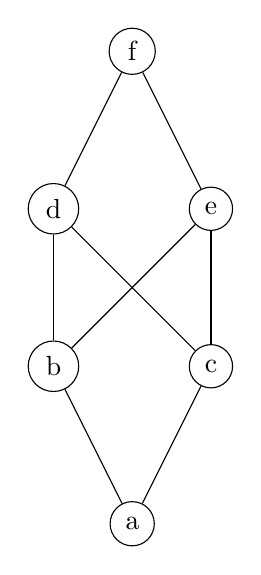
\begin{tikzpicture}

      \begin{scope}[every node/.style={circle,draw}]
        \node (f)  at (1,6)  {f};
        \node (e)  at (2,4)  {e};
        \node (d)  at (0,4)  {d};
        \node (c)  at (2,2)  {c};
        \node (b)  at (0,2)  {b};
        \node (a)  at (1,0)  {a};
      \end{scope}

      \begin{scope}[every node/.style={fill=white,circle}]

        \begin{scope}[every edge/.style={draw}]
          \path (a)  edge (b);
          \path (a)  edge (c);
          \path (b)  edge (d);
          \path (b)  edge (e);
          \path (c)  edge (d);
          \path (c)  edge (e);
          \path (d)  edge (f);
          \path (e)  edge (f);

        \end{scope}
      \end{scope}

    \end{tikzpicture}
    \caption{Not a lattice: the infinimum of $d$ and $e$ is not unique}
  \end{center}
\end{figure}

\begin{definition}[Bounded poset]
  \index{bounded poset}
\end{definition}

\begin{definition}[Ranked poset]
  \index{ranked poset}
  A poset is \textit{ranked} if there exists a function: $\rank : P \to \mathbb Z$ such that
  \begin{enumerate}
    \item if $x < y$, then $\rank(x) < \rank(y)$ $(x, y \in P)$
    \item if $x < y$ and if there exists no $z \in P$ such that $x < z < y$, then $\rank(y) = \rank(x) + 1$ $(x, y \in R)$.
  \end{enumerate}
\end{definition}

\paragraph{}
On the Hasse diagram, it means that, if we place all elements with the same rank at the same level, an element in only connected to elements placed the level just above or just under itself.


\begin{figure}[H]
  \begin{center}
    \begin{tikzpicture}

      \node at (-4,6) {$r = 3$};
      \node at (-4,4) {$r = 2$};
      \node at (-4,2) {$r = 1$};
      \node at (-4,0) {$r = 0$};

      \draw[very thin, dashed] (-3,6) -- (5,6);
      \draw[very thin, dashed] (-3,4) -- (5,4);
      \draw[very thin, dashed] (-3,2) -- (5,2);
      \draw[very thin, dashed] (-3,0) -- (5,0);

      \begin{scope}[every node/.style={circle,draw,fill=white}]
        \node (f)  at (1,6)  {f};
        \node (e)  at (2,4)  {e};
        \node (d)  at (0,4)  {d};
        \node (c)  at (2,2)  {c};
        \node (b)  at (0,2)  {b};
        \node (a)  at (1,0)  {a};
      \end{scope}

      \begin{scope}[every node/.style={fill=white,circle}]

        \begin{scope}[every edge/.style={draw}]
          \path (a) edge (b);
          \path (a) edge (c);
          \path (b) edge (d);
          \path (b) edge (e);
          \path (c) edge (d);
          \path (c) edge (e);
          \path (d) edge (f);
          \path (e) edge (f);

        \end{scope}
      \end{scope}

    \end{tikzpicture}
    \caption{Poset with rank indication}
  \end{center}
\end{figure}

\begin{proposition}
  Let $(P,\le)$ be a bounded poset, then it's ranked if and only if all it's maximal chain of the same length.
\end{proposition}
